\section{El proceso de las indicaciones}

Para estilizar la secuencia de votación e indicación de un proyecto, consideramos un ejemplo simple. Se introduce un proyecto que contiene tres artículos. 

\begin{itemize}
\item Art 1. Se abre partida de \$200
\item Art 2. Se la divide por mitades
\item Art 3. Una mitad para alumnos, la otra para maestros
\end{itemize}

\noindent Si se aprobara, habría \$100 para maestros y alumnos. Si la mayoría quisiera entregarle \$150 a los maestros, podría hacer una indicación al art.\ 1, aumentando la partida a \$300. Problema: el único que puede hacerla en Chile es el ejecutivo. Si Hacienda se negase a gastar más, aún queda la ruta distributiva: menos para los alumnos, más para los maestros. Basta una enmienda al segundo artículo para dejar la distribución en $\frac{1}{3}$ y $\frac{2}{3}$. 

Notación:
\begin{itemize}
\item $p$ es el proyecto
\item $q$ es el status quo (todos reciben \$0)
\item $p_1$ es proyecto con art.\ 1 indicado
\item $p_2$ es proyecto con art.\ 2 indicado
\item $p_{12}$ es proyecto con arts.\ 1 y 2 indicados
\end{itemize}

La negociación procede así. Si la comisión de Hacienda admitiera la indicación al art.\ 1, el primer informe contaría con el proyecto $p$ y la versión modificada $p_1$. La discusión en general es un voto $p$ vs.\ $q$ primero. Si ganara $p$ (en algunos casos por supermayoría), seguiría un voto por la adminisilidad de la indicación, resultando $p1$ si ganara, $p$ si perdiera.

Regresa a comisión para un segundo informe. En él, se podría introducir la enmienda del art.\ 2, o $p_2$. La Figura \ref{f:agendaUrg} estiliza el proceso. Lo fundamental es que las urgencias sumas y de discusión inmediata (en Cámara, por lo menos) hacen que se prescinda del segundo informe y su duscusión. Así que urgencia = closed rule. [Hay que regresar a ley org. y reglamento para ver si la caricatura es acertada.]

Un perfil de preferencia para ilustrar podria ser:
\begin{itemize}
\item La mayoría está cerca de los maestros y ordena las alternativas $p_{12}>p_{2}>p_{1}>p>q$ (de mejor a peor)
\item El gobierno:  $p>q>p_2>p_1>p_{12}$.
\end{itemize}




\begin{sidewaysfigure}
  \centering
    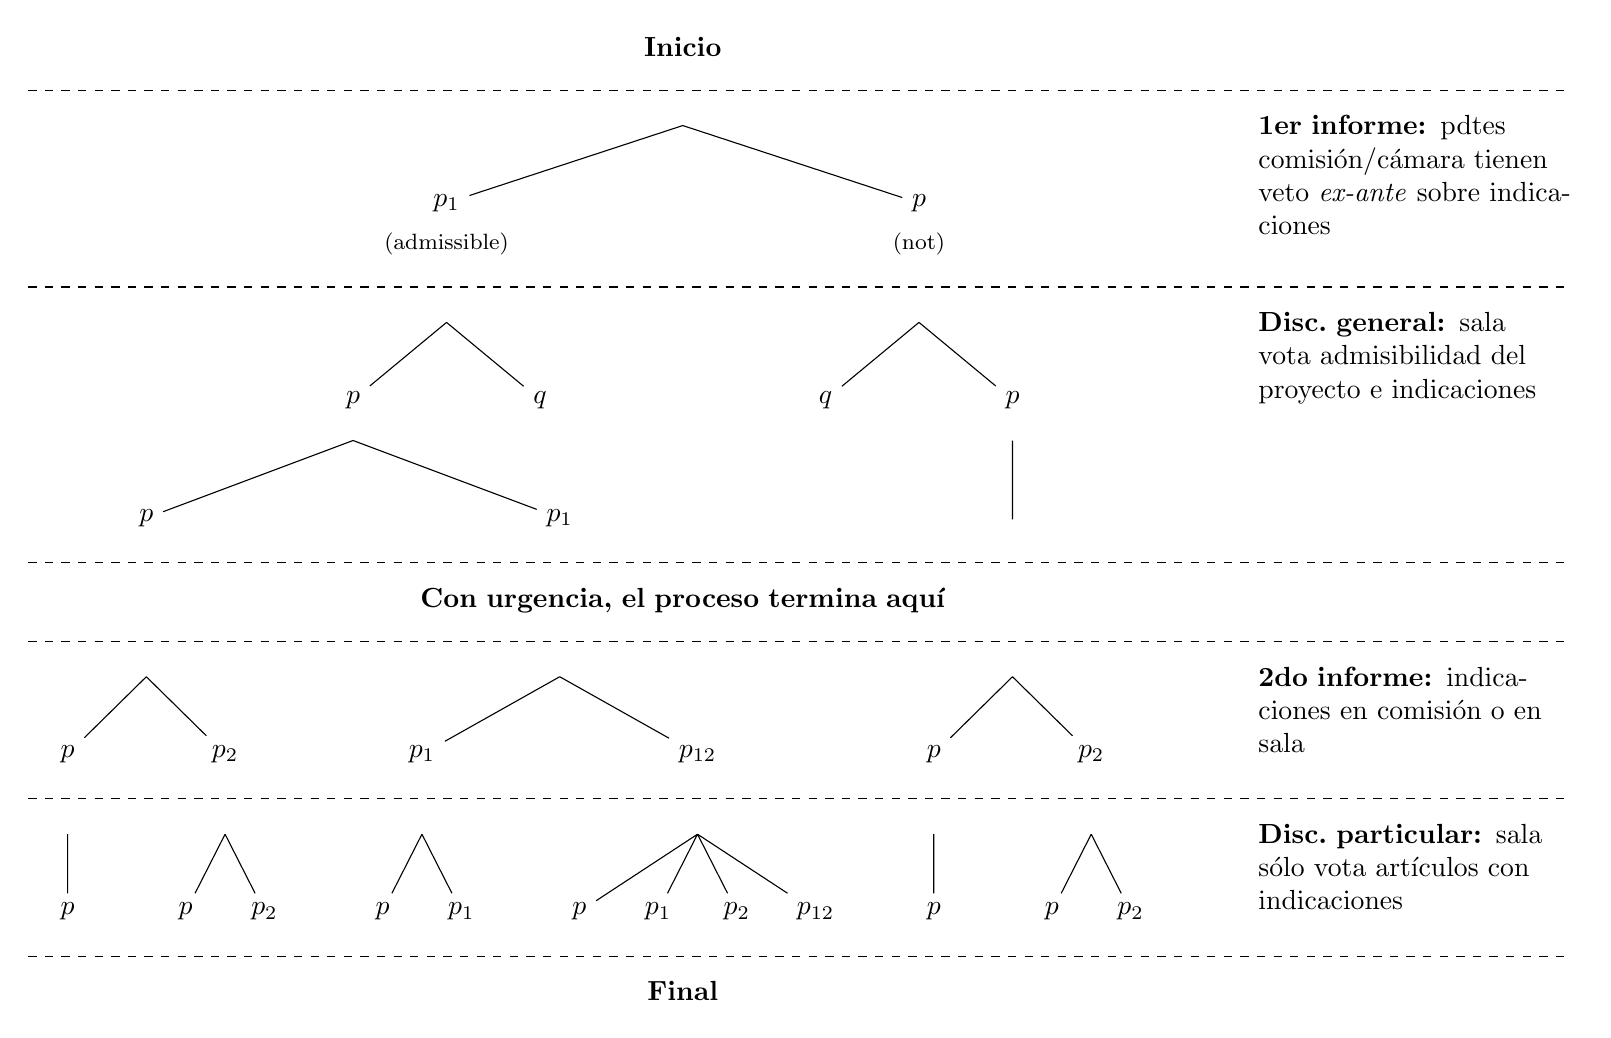
\begin{tikzpicture}
      \node[text width=10cm, text centered, anchor=north,fill=white] at (8.8125,-11) {\textbf{Final}}; 
      %%%%%%%%%%%%%%%%%%%%%%%%%%%%%%%%%%%%%%%%%%%%%%%
      \draw[dashed] (0.5,-10.8) -- (20,-10.8);
      %%%%%%%%%%%%%%%%%%%%%%%%%%%%%%%%%%%%%%%%%%%%%%%
      \node[below] at (1,-10)    (o1)  {$p$}; 
      \node[below] at (2.5,-10)  (o2)  {$p$}; 
      \node[below] at (3.5,-10)  (o3)  {$p_2$}; 
      \node[below] at (5,-10)    (o4)  {$p$}; 
      \node[below] at (6,-10)    (o5)  {$p_1$}; 
      \node[below] at (7.5,-10)  (o6)  {$p$}; 
      \node[below] at (8.5,-10)  (o7)  {$p_1$}; 
      \node[below] at (9.5,-10)  (o8)  {$p_2$}; 
      \node[below] at (10.5,-10) (o9)  {$p_{12}$}; 
      \node[below] at (12,-10)   (o10) {$p$}; 
      \node[below] at (13.5,-10) (o11) {$p$}; 
      \node[below] at (14.5,-10) (o12) {$p_2$}; 
      \draw (1,-9.25) -- (o1)
            (3,-9.25) -- (o2)
            (3,-9.25) -- (o3)
            (5.5,-9.25) -- (o4)
            (5.5,-9.25) -- (o5)
            (9,-9.25) -- (o6)
            (9,-9.25) -- (o7)
            (9,-9.25) -- (o8)
            (9,-9.25) -- (o9)
            (12,-9.25) -- (o10)
            (14,-9.25) -- (o11)
            (14,-9.25) -- (o12);
      \draw[dashed] (0.5,-8.8) -- (20,-8.8);
      \node[text width=4cm, anchor=north west,fill=white] at (16,-9) {\textbf{Disc.\ particular:} sala sólo vota artículos con indicaciones}; 
      %%%%%%%%%%%%%%%%%%%%%%%%%%%%%%%%%%%%%%%%%%%%%%%
      \node[below] at (1,-8) (i21) {$p$}; 
      \node[below] at (3,-8) (i22) {$p_2$}; 
      \node[below] at (5.5,-8) (i23) {$p_1$}; 
      \node[below] at (9,-8) (i24) {$p_{12}$}; 
      \node[below] at (12,-8) (i25) {$p$}; 
      \node[below] at (14,-8) (i26) {$p_2$}; 
      \draw (2,-7.25) -- (i21)
            (2,-7.25) -- (i22)
            (7.25,-7.25) -- (i23)
            (7.25,-7.25) -- (i24)
            (13,-7.25) -- (i25)
            (13,-7.25) -- (i26);
      \draw[dashed] (0.5,-6.8) -- (20,-6.8);
      \node[text width=4cm, anchor=north west,fill=white] at (16,-7) {\textbf{2do informe:} indicaciones en comisión o en sala}; 
      % %%%%%%%%%%%%%%%%%%%%%%%%%%%%%%%%%%%%%%%%%%%%%%%
      \draw[dashed] (0.5,-5.8) -- (20,-5.8);
      \node[text width=10cm, text centered, anchor=north,fill=white] at (8.8125,-6) {\textbf{Con urgencia, el proceso termina aquí}}; 
      %%%%%%%%%%%%%%%%%%%%%%%%%%%%%%%%%%%%%%%%%%%%%%%
      \node[below] at (2,-5) (g11) {$p$}; 
      \node[below] at (7.25,-5) (g12) {$p_1$}; 
      \node[below] at (4.625,-3.5) (g1) {$p$}; 
      \node[below] at (7,-3.5) (g2) {$q$}; 
      \node[below] at (13,-3.5) (g3) {$p$}; 
      \node[below] at (10.625,-3.5) (g4) {$q$}; 
      \draw (4.625,-4.25) -- (g11)
            (4.625,-4.25) -- (g12)
            (13,-4.25) -- (13,-5.25)
            (5.8125,-2.75) -- (g1)
            (5.8125,-2.75) -- (g2)
            (11.8125,-2.75) -- (g3)
            (11.8125,-2.75) -- (g4);
      \draw[dashed] (0.5,-2.3) -- (20,-2.3);
      \node[text width=4cm, anchor=north west,fill=white] at (16,-2.5) {\textbf{Disc.\ general:} sala vota admisibilidad del proyecto e indicaciones}; 
      %%%%%%%%%%%%%%%%%%%%%%%%%%%%%%%%%%%%%%%%%%%%%%%
      \node[below] at (5.8125,-1) (i11) {$p_1$}; 
      \node[text width=2cm, text centered] at (5.8125,-1.75) {\footnotesize{(admissible)}}; 
      \node[below] at (11.8125,-1) (i12) {$p$}; 
      \node[text width=2cm, text centered] at (11.8125,-1.75) {\footnotesize{(not)}}; 
      \draw (8.8125,-.25) -- (i11)
            (8.8125,-.25) -- (i12);
      \draw[dashed] (0.5,.2) -- (20,.2);
      \node[text width=4cm, anchor=north west,fill=white] at (16,0) {\textbf{1er informe:} pdtes comisión/cámara tienen veto \emph{ex-ante} sobre indicaciones}; 
      %%%%%%%%%%%%%%%%%%%%%%%%%%%%%%%%%%%%%%%%%%%%%%%
      \node[text width=10cm, text centered, anchor=north,fill=white] at (8.8125,1) {\textbf{Inicio}}; 
      %%%%%%%%%%%%%%%%%%%%%%%%%%%%%%%%%%%%%%%%%%%%%%%
    \end{tikzpicture}  \\
\caption{Stylization of the voting agenda. Notación: $p$ es un proyecto; $q$ el status quo; $p_1$, $p_2$ y $p_{12}$ son, respectivamente, enmiendas al primer artículo del proyecto, al segundo o a ambos. Vea el texto.}\label{f:agendaUrg}
\end{sidewaysfigure}
